%% start of file `cv_german.tex', based on `template_en.tex` by Xavier Danaux (xdanaux@gmail.com).
% This work may be distributed and/or modified under the
% conditions of the LaTeX Project Public License version 1.3c,
% available at http://www.latex-project.org/lppl/.
% 
% Thomas Quaritsch <t.quaritsch@student.tugraz.at>

\documentclass[11pt,a4paper]{moderncv}

\usepackage[german]{babel}
\usepackage{moderncv-additions}

% moderncv themes
\moderncvtheme{casual}   % optional arguments are 'blue' (default), 'orange', 'red', 'green', 'grey' and 'roman' (for roman fonts, instead of sans serif fonts)
%\moderncvtheme[green]{classic}                % idem

% character encoding
\usepackage[utf8]{inputenc}                   % replace by the encoding you are using

% adjust the page margins
\usepackage[scale=0.8]{geometry}
\setlength{\hintscolumnwidth}{3cm}			  % if you want to change the width of the column with the dates
%\AtBeginDocument{\setlength{\maketitlenamewidth}{6cm}}  % only for the classic theme, if you want to change the width of your name placeholder (to leave more space for your address details

\usepackage[dvipsnames]{xcolor}

\AtBeginDocument{\recomputelengths}           % required when changes are made to page layout lengths

% personal data
\firstname{Patrick}
\familyname{Grüner}
%\title{Resumé title (optional)}              
\address{Jahnstraße 5}{87700 Memmingen}        
\mobile{+49 176 47705895}                     
%\phone{phone (optional)}                      
\email{patrick.gmm91@gmail.com}                      
\photo[64pt]{picture}                          % '64pt' is the height the picture must be resized to and 'picture' is the name of the 
\quote{``Das ist ein toller Frusterspruch\\ von Friede Frusterfrau.'' -- Friede Frusterfrau}                 

%\nopagenumbers{}                             % uncomment to suppress automatic page numbering for CVs longer than one page

%----------------------------------------------------------------------------------
%            content
%----------------------------------------------------------------------------------

\begin{document}

% color redefinitions must be after \begin{document}!
%Liebherr yellow {253,196,0} black {0,0,0}
%Multivac {0, 105, 180}
%Rhode {0,60,124}
%Grob {0,58,121}
%Boeringer {1,51,103}
\definecolor{firstnamecolor}{RGB}{0,0,0}
\definecolor{familynamecolor}{RGB}{0,0,0}
\definecolor{quotecolor}{RGB} {1,51,103}
\definecolor{addresscolor}{RGB}{0,0,0}
\definecolor{sectionrectanglecolor}{RGB}{1,51,103}
\definecolor{sectiontitlecolor}{RGB}{1,51,103}
\definecolor{subsectioncolor}{RGB}{1,51,103}
\definecolor{footersymbolcolor}{RGB}{0,0,0}

\makeatletter

%\pagestyle{empty}
%\chapter*{Bewerbungs}{unterlagen}
%
%\vspace*{50mm}
%\begin{minipage}{\textwidth}
%	\vspace*{3mm}
%	\familynamestyle{\@firstname}~~\firstnamestyle{\@familyname} 	
%	\hspace*{5mm}{{\color{firstnamecolor}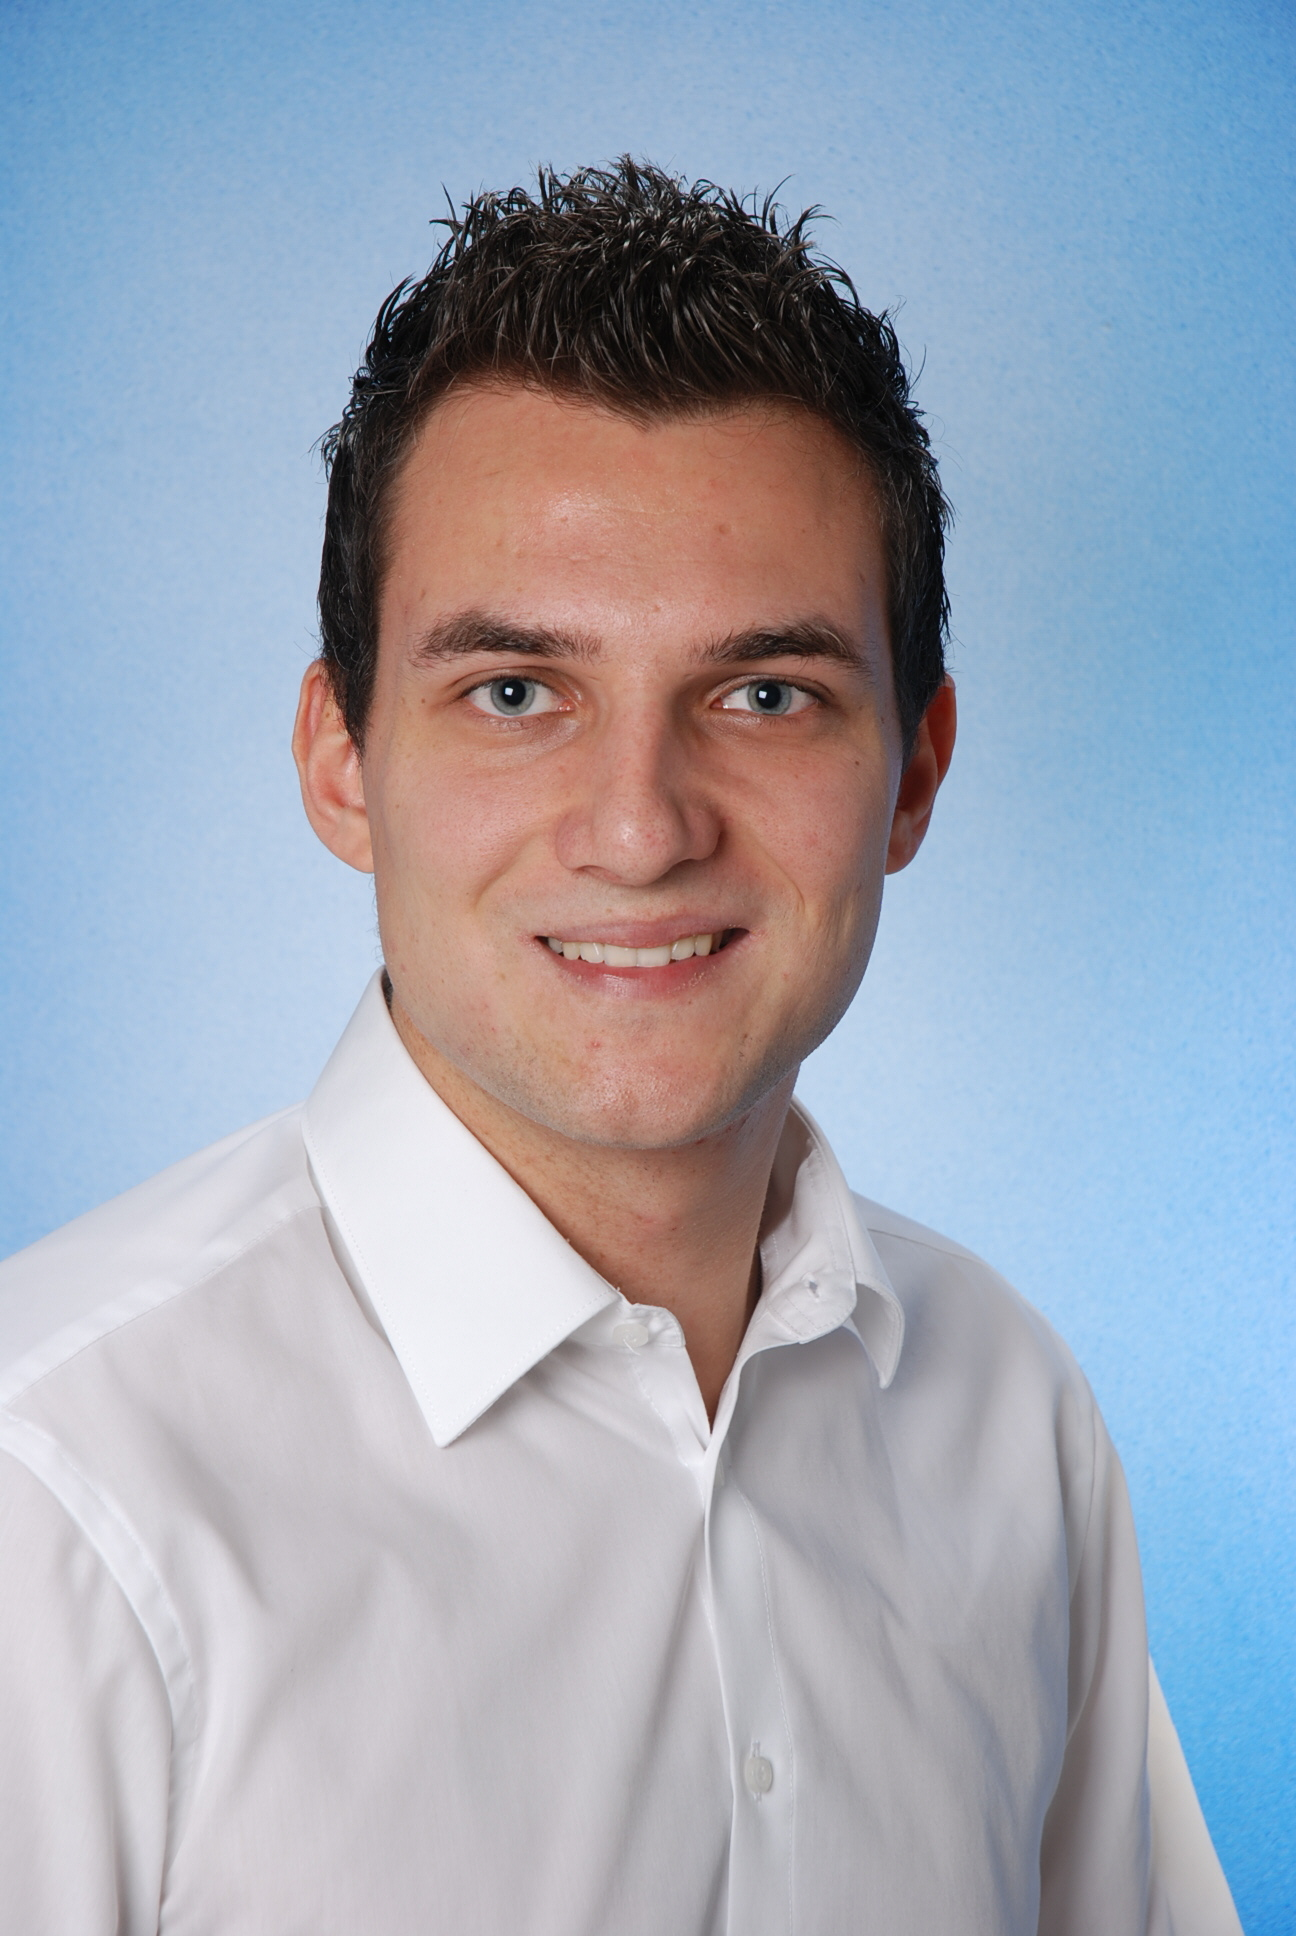
\includegraphics[width=128pt]{Anlagen/picture}}}\\[3mm]
%	\@addressstreet, \@addresscity ~~~ \mobilesymbol~\@mobile ~~~ \emailsymbol~\@email
%\end{minipage}
%\begin{minipage}{70pt}
%	
%\end{minipage}
%
%\vfill
%
%\begin{minipage}{1.0\textwidth}
%	\section{Inhalt}
%	\tableofcontents
%\end{minipage}
%
%\newpage
\pagestyle{fancy}

\chapter{Lebenslauf}{}
%\makequote

\section{Persönliche Daten}
%%%%%%%%%%%%%%%%%%%%%%%%%%%%%%%%%%%%%%%%%%%%%%%%%%%%%%%%%%%%%%%%%%%%
\cvline{Name}{\@firstname~\@familyname}
\cvline{Anschrift}{\@addressstreet, \@addresscity}
\cvline{Telefon}{\@mobile}
\cvline{E-Mail}{\@email}
\cvline{Geburtsdaten}{12.09.1991 in Memmingen}
\cvline{Staatsbürgerschaft}{Deutsch}
%\cvline{Führerschein}{A,B,C,D,E,F,G}
\makeatother 

%\cventry{year--year}{Degree}{Institution}{City}{\textit{Grade}}{Description}  % arguments 3 to 6 are optional


\section{Berufliche Laufbahn} 
%%%%%%%%%%%%%%%%%%%%%%%%%%%%%%%%%%%%%%%%%%%%%%%%%%%%%%%%%%%%%%%%%%%%

\cventry{06/2018 -- heute}{Projektleiter/Softwareentwickler}{Liebherr Verzahntechnik GmbH}{Kempten}{}
{ Projektleitung und Hauptverantwortlichkeit für Bildverarbeitungs- und Technologielösungen im Bereich Automation, Weiterentwicklung und Wartung der Software \textcolor{RoyalBlue}{\href{https://www.youtube.com/watch?v=-PjGzlYVw8U}{LHRobotics.Vision}}, Projektleitung und Beteiligungen an staatlich geförderten Forschungsprojekten}  % arguments 3 to 6 are optional

\section{Akademische Laufbahn} 
%%%%%%%%%%%%%%%%%%%%%%%%%%%%%%%%%%%%%%%%%%%%%%%%%%%%%%%%%%%%%%%%%%%%

\cventry{10/2015 -- 06/2018}{Master Informatik}{Universität}{Augsburg}{\textit{M.Sc}}{Note: 1,9}  % arguments 3 to 6 are optional

\cventry{10/2011 -- 08/2015}{Bachelor Informatik}{Fachhochschule}{Kempten}{\textit{B.Sc}}{Note: 2,4} 

\section{Sonstige Erfahrungen} 
%%%%%%%%%%%%%%%%%%%%%%%%%%%%%%%%%%%%%%%%%%%%%%%%%%%%%%%%%%%%%%%%%%%%
\cventry{11/2017 -- 06/2018}{Masterarbeit}{CMORE Automotive GmbH}{}{}{Entwicklung einer Virtual Reality Applikation mittels der Unity-.NET Umgebung zur Annotierung von 3D-Punktwolken}
%\cventry{10/2017 -- 02/2018}{Projektarbeit}{Universität Augsburg}{}{}{Entwicklung einer Augmented Reality Applikation für die Microsoft Hololens AR-Brille mittels der Unity-.NET Umgebung, um elektrische Felder von kapazitiven Sensoren holographisch darzustellen}
\cventry{04/2017 -- 11/2017}{Audi Autonomous Driving Cup}{Universität Augsburg}{}{}{Entwicklung von vollautomatischen Fahrfunktionen und die dafür notwendigen Software-Architekturen innerhalb von C++-ADTF-Filtern für Audi-Q2-Modellfahrzeuge innerhalb des Uni-Augsburg Teams %im Maßstab 1:8
}
\cventry{03/2016 -- 07/2016}{Praktikum}{Universität Augsburg}{}{}{Entwicklung von C-basierten Mikrocontroller Programmen zur Steuerung von mobilen iRobot Roomba Robotern}
\cventry{04/2015 -- 08/2015}{Bachelorarbeit}{Christ Elektronik GmbH}{Memmingen}{}{Analyse und Entwicklung eines Prototypen zur Portierung der, mit der Entwicklungsumgebung \dq VisBee\dq{} erstellten, .NET-Touch-Panel-Anwendungen unter Linux}
%\cventry{04/2014 -- 07/2014}{Projektarbeit}{Fachhochschule Kempten}{}{}{Entwicklung einer Zahnputzassistenz-Applikation für mobile Android Geräte}
\cventry{09/2013 -- 02/2014}{Praxissemester}{Liebherr Aerospace GmbH}{Lindenberg}{}{Inbetriebnahme und Analyse der Testumgebung 
\dq YAVE\dq{} für den Software High-Level Test}

\newpage
\section{Schulische Laufbahn} 
%%%%%%%%%%%%%%%%%%%%%%%%%%%%%%%%%%%%%%%%%%%%%%%%%%%%%%%%%%%%%%%%%%%%

\cventry{09/2008 -- 07/2011}{Fachoberschule}{}{Memmingen}{Schwerpunkt: Technik}{Note: 2,8}
\cventry{09/2003 -- 07/2008}{Gymnasium}{}{Buxheim}{}{}

\section{IT Kompetenzen} 
%%%%%%%%%%%%%%%%%%%%%%%%%%%%%%%%%%%%%%%%%%%%%%%%%%%%%%%%%%%%%%%%%%%%

\cvline{Programmiersprachen}{C++ und C\#(gut), Lua (gut)}
\cvline{IDEs}{Visual Studio, CoppeliaSim, Halcon HDevelop}
\cvline{Office}{Word, \LaTeX , Powerpoint, Outlook, Excel, Photoshop}

\section{Sprachen} 
%%%%%%%%%%%%%%%%%%%%%%%%%%%%%%%%%%%%%%%%%%%%%%%%%%%%%%%%%%%%%%%%%%%%

\cvline{Deutsch}{Muttersprache}{}
\cvline{Englisch}{Fließend in Wort und Schrift}

%\section{Hobbys}
%%%%%%%%%%%%%%%%%%%%%%%%%%%%%%%%%%%%%%%%%%%%%%%%%%%%%%%%%%%%%%%%%%%%

%\cvline{}{Basketball}
%\cvline{}{Kraftsport}
%\cvline{}{Taekwondo}

\newpage

%\section{Auszeichnungen} 
%%%%%%%%%%%%%%%%%%%%%%%%%%%%%%%%%%%%%%%%%%%%%%%%%%%%%%%%%%%%%%%%%%%%

%\section{Außeruniversitäre Tätigkeiten} 
%%%%%%%%%%%%%%%%%%%%%%%%%%%%%%%%%%%%%%%%%%%%%%%%%%%%%%%%%%%%%%%%%%%%

%\section{Publikationen} 
%%%%%%%%%%%%%%%%%%%%%%%%%%%%%%%%%%%%%%%%%%%%%%%%%%%%%%%%%%%%%%%%%%%%
%\subsection{Konferenzen und Workshops}
%\cvline{mm/jjjj}{Autor 1 und Autor 2. \textbf{Mustertitel: Unser tolles Paper.} In \textit{Proceedings of the First Muster Workshop %1970}, Musterstadt, Musterland, YYYY.}

% \newpage

%\subsection{Technical Reports}

%\cvline{....}{....}

%\cvline{....}{alternativ kann man auch BibTex verwenden:}

%\renewcommand*{\refname}{Abschlussarbeiten}
%\nocite{*}
%\bibliographystyle{cv}
%\bibliography{publications}       % 'publications' is the name of a BibTeX file

%\newpage
%\chapter{AADC}{}
%\vspace*{1cm}
%\begin{center}
%	 \fbox{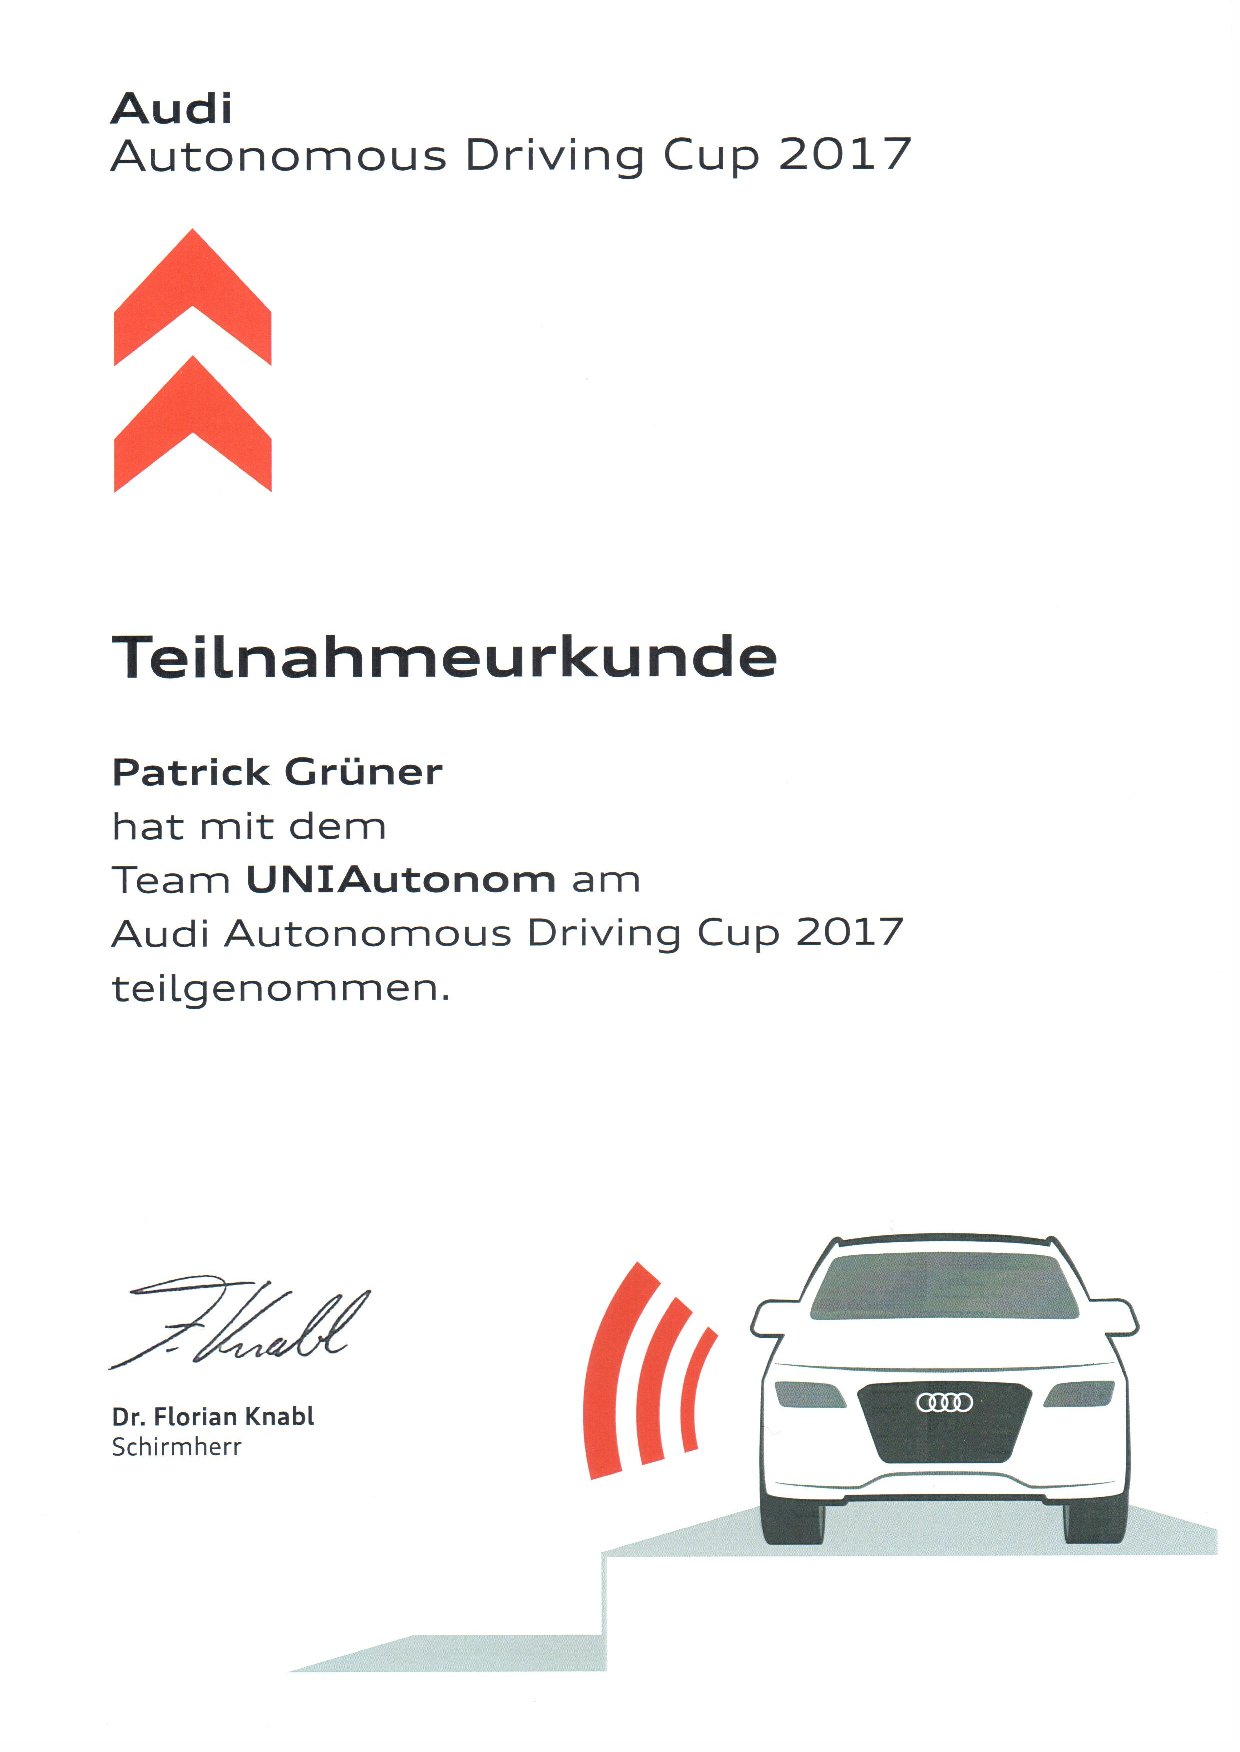
\includegraphics[height=0.85\textheight]{Anlagen/AADC}}	
%\end{center}
%
%\chapter{Bachelor}{}
%\vspace*{1cm}
%\begin{center}
%	 \fbox{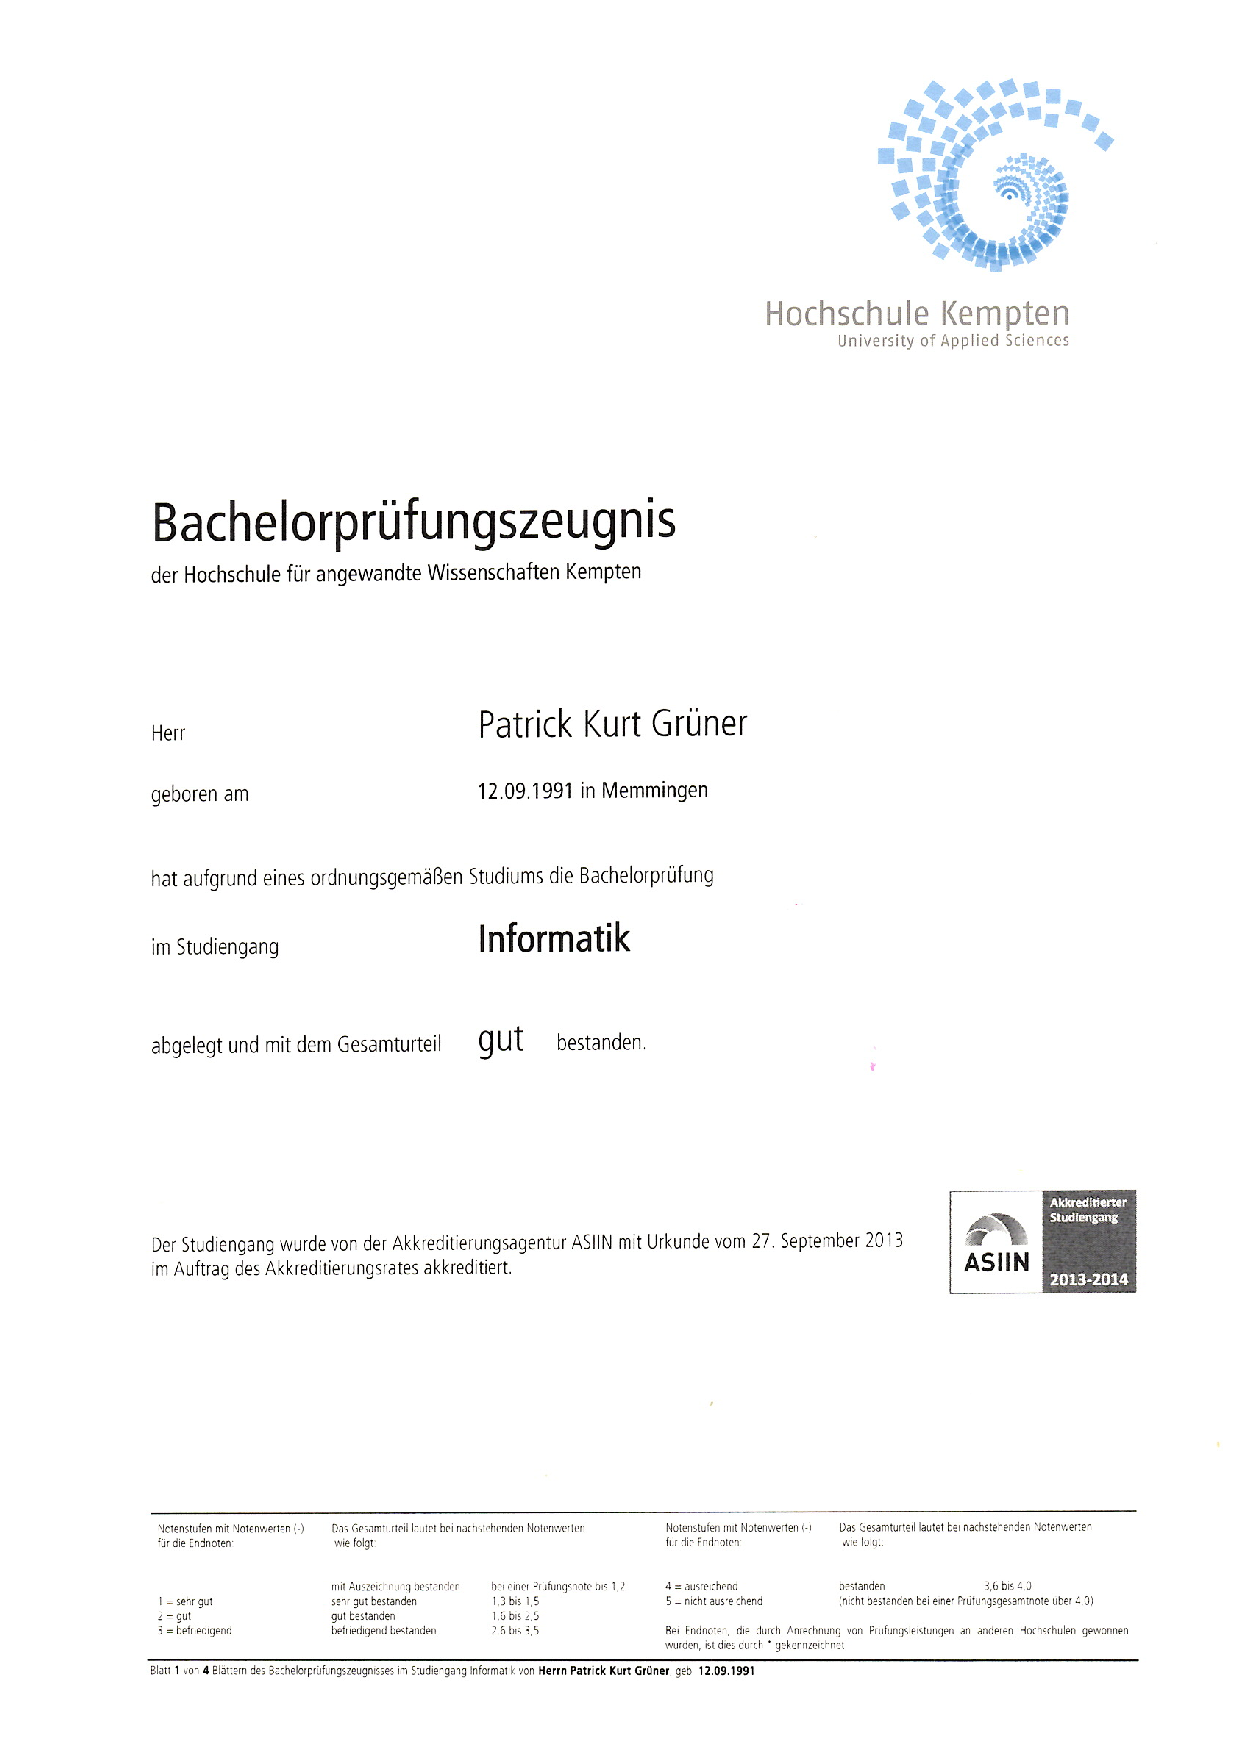
\includegraphics[height=0.85\textheight]{Anlagen/Bachelorzeugnis}}	
%\end{center}
%
%\newpage
%\chapter{Praxissemester}{}
%\vspace*{1cm}
%\begin{center}
%	\fbox{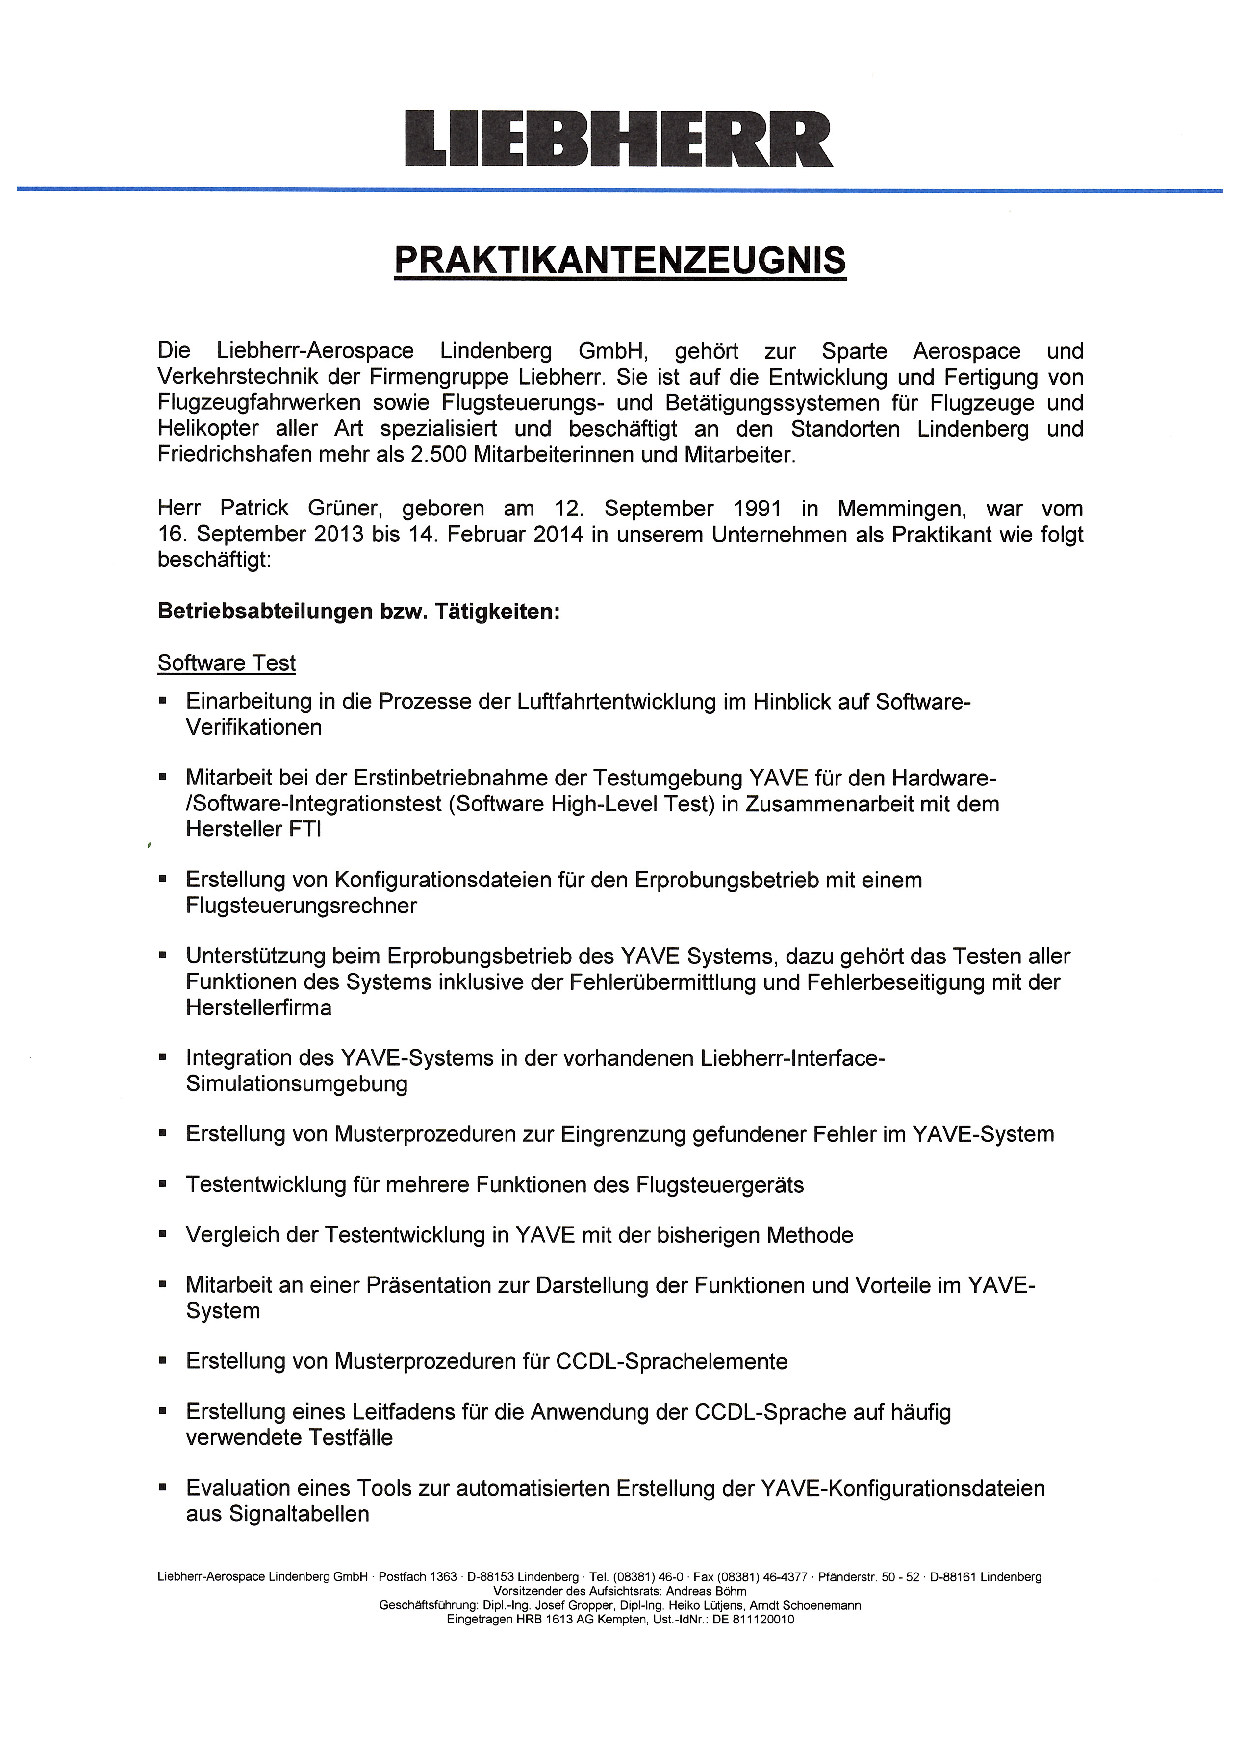
\includegraphics[height=0.85\textheight]{Anlagen/PraktikumLiebherr1}}		
%\end{center}
%
%\vspace*{1cm}
%\begin{center}
%	\fbox{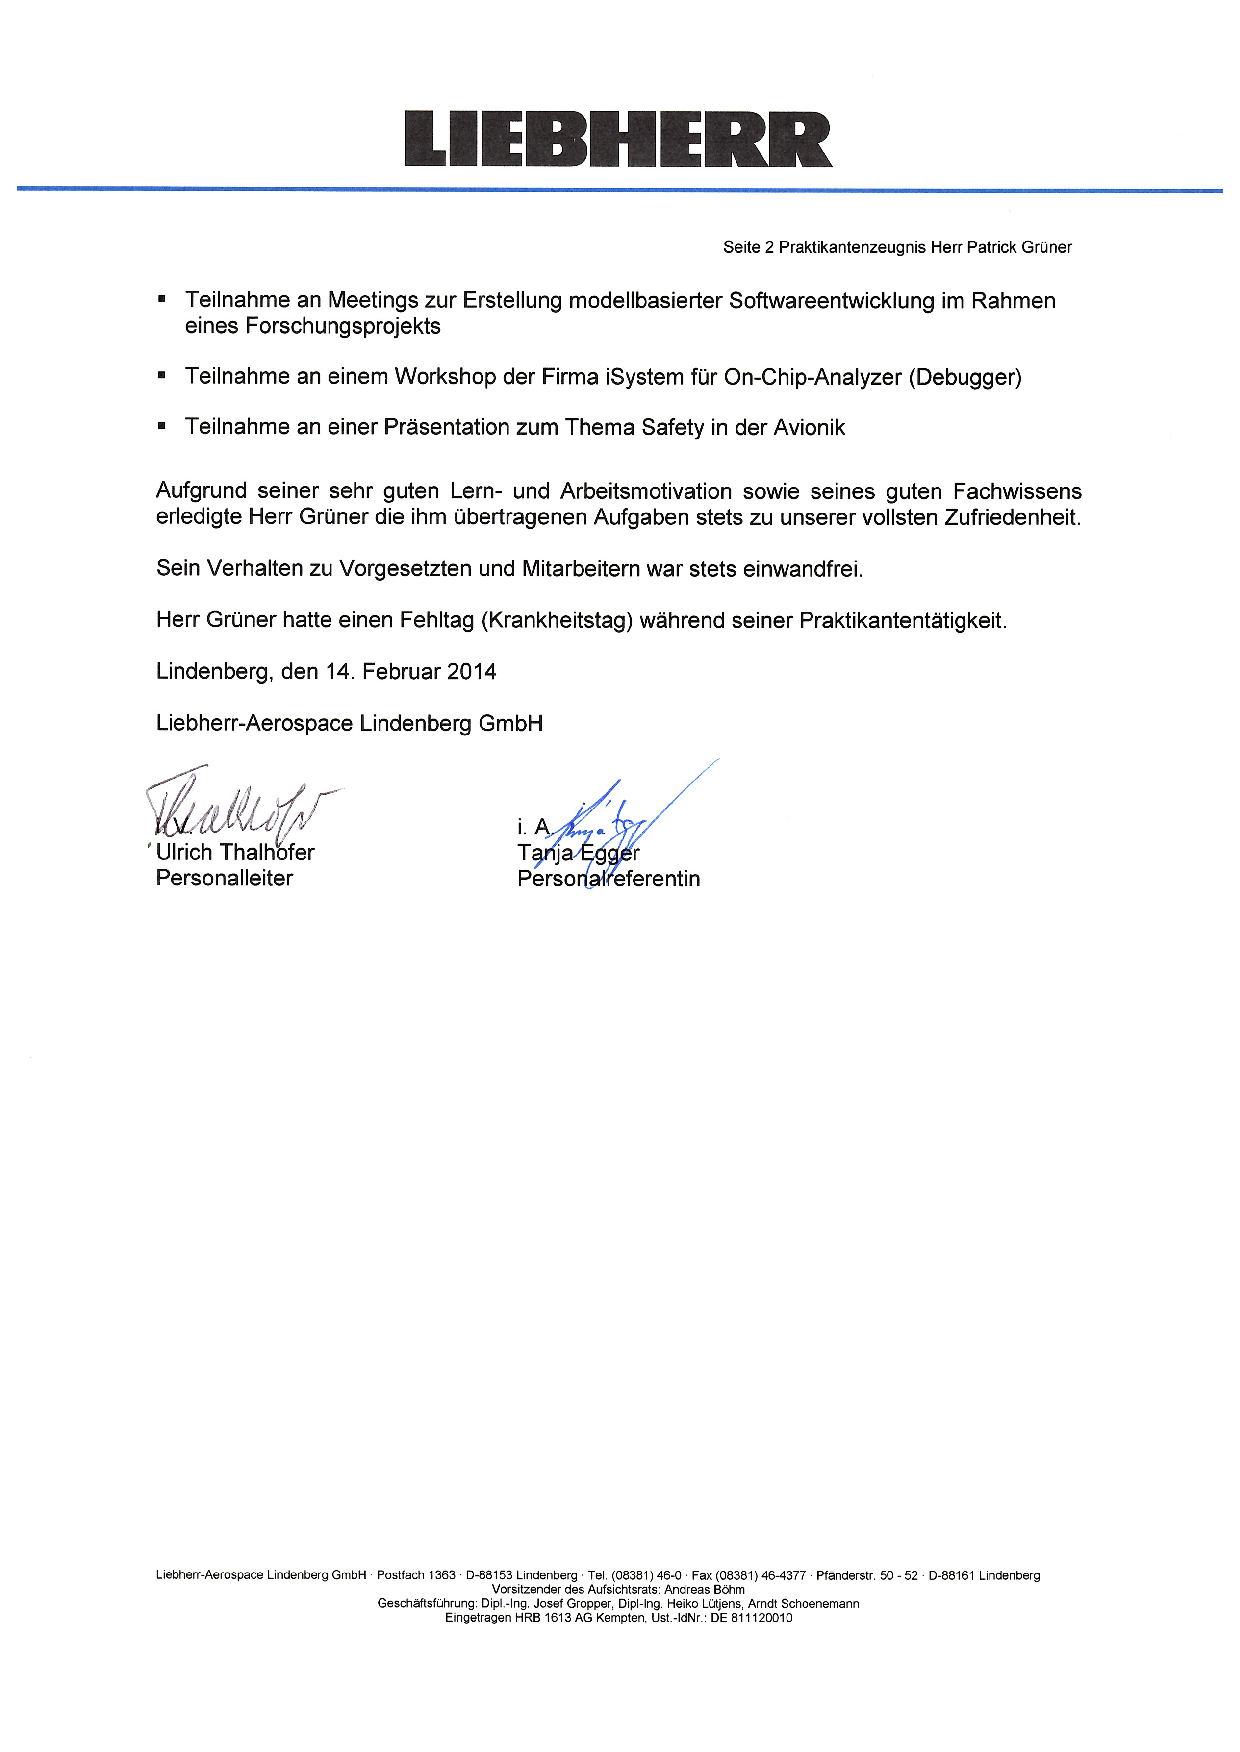
\includegraphics[height=0.85\textheight]{Anlagen/PraktikumLiebherr2}}	
%\end{center}
%
% \newpage
%\chapter{Abitur}{}
% \vspace*{1cm}
% \begin{center}
% 	\fbox{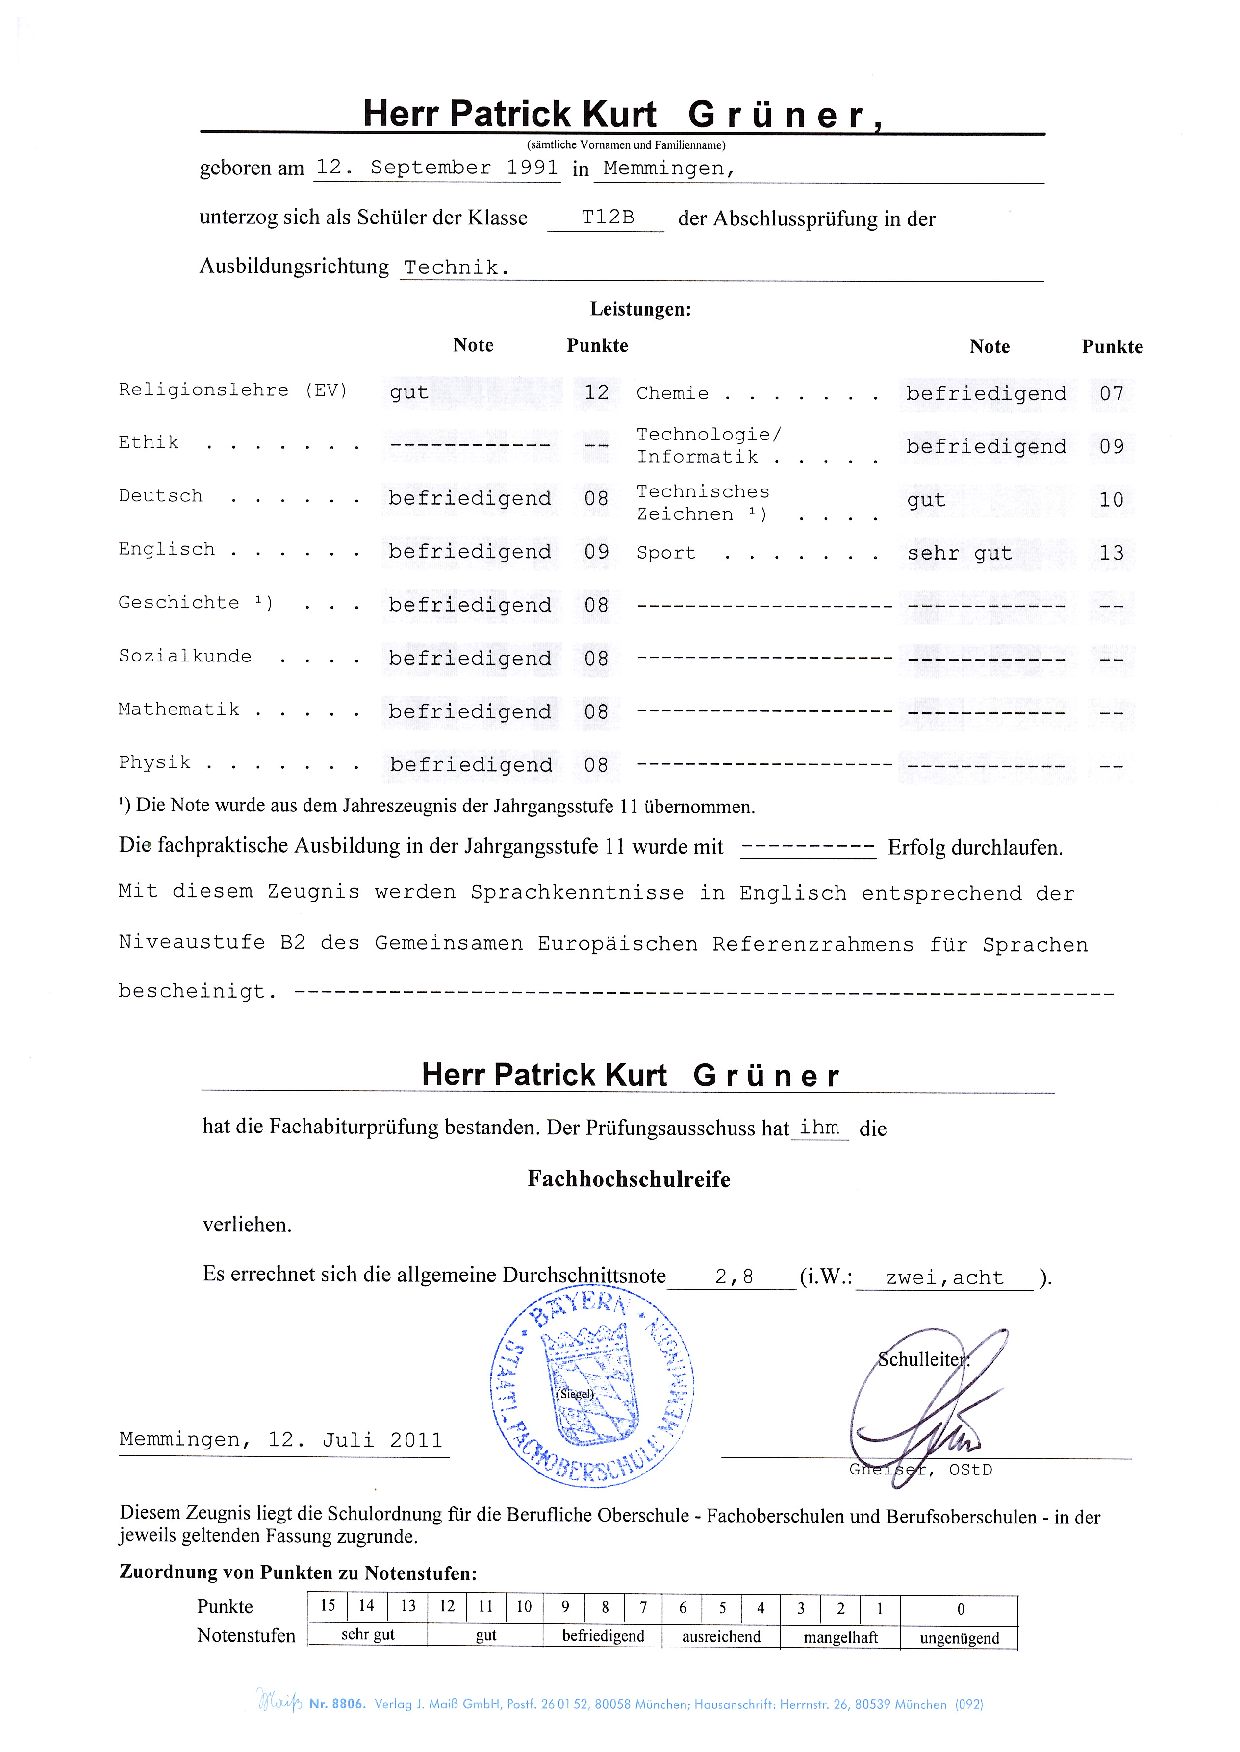
\includegraphics[height=0.85\textheight]{Anlagen/Abizeugnis}}	
% \end{center}

\end{document}

% end of file `cv_german.tex'